\documentclass[preprint]{elsarticle}

\usepackage{lineno,hyperref}
\modulolinenumbers[5]


\usepackage{physics}
\usepackage{graphicx,amsmath,amssymb,mathtools,hyperref,amsfonts,pgfplots,caption,epstopdf,todonotes,tikz,subcaption}
\usepackage{siunitx}
\usepackage[version=4]{mhchem}

\usetikzlibrary{patterns}
\usetikzlibrary{arrows}
\pgfplotsset{compat=1.13}

\newcommand{\tino}[1]{\todo[inline,color=red!40]{Tino: #1}}
\newcommand{\scott}[1]{\todo[inline,color=green!40]{Scott: #1}}

\journal{Journal of Power Sources}

%%%%%%%%%%%%%%%%%%%%%%%
%% Elsevier bibliography styles
%%%%%%%%%%%%%%%%%%%%%%%
%% To change the style, put a % in front of the second line of the current style and
%% remove the % from the second line of the style you would like to use.
%%%%%%%%%%%%%%%%%%%%%%%

%% Numbered
%\bibliographystyle{model1-num-names}

%% Numbered without titles
%\bibliographystyle{model1a-num-names}

%% Harvard
%\bibliographystyle{model2-names.bst}\biboptions{authoryear}

%% Vancouver numbered
%\usepackage{numcompress}\bibliographystyle{model3-num-names}

%% Vancouver name/year
%\usepackage{numcompress}\bibliographystyle{model4-names}\biboptions{authoryear}

%% APA style
%\bibliographystyle{model5-names}\biboptions{authoryear}

%% AMA style
%\usepackage{numcompress}\bibliographystyle{model6-num-names}

%% `Elsevier LaTeX' style
\bibliographystyle{elsarticle-num}
%%%%%%%%%%%%%%%%%%%%%%%

%% Put any plot commands in here 

% noniso{D, nx, ylim} 

%\definecolor{c1}{RGB}{102,194,165}
%\definecolor{c2}{RGB}{252,141,98}
%\definecolor{c3}{RGB}{141,160,203}
%\definecolor{c4}{RGB}{231,138,195}
%\definecolor{c5}{RGB}{166,216,84}
%\definecolor{c6}{RGB}{255,217,47}

\definecolor{c1}{RGB}{228,26,28}
\definecolor{c2}{RGB}{55,126,184}
\definecolor{c3}{RGB}{77,175,74}
\definecolor{c4}{RGB}{152,78,163}
\definecolor{c5}{RGB}{255,127,0}
\definecolor{c6}{RGB}{106,61,154}


\pgfplotscreateplotcyclelist{mylist}{
{c1,thick}, 
{c2,thick},
{c3,thick},
{c4,thick},
{c5,thick},
{c1,dashed,thick},
{c1,dotted,thick},
{c2,dashed,thick},
{c2,dotted,thick},
{c3,dashed,thick},
{c3,dotted,thick},
{c4,dashed,thick},
{c4,dotted,thick},
{c5,dashed,thick},
{c5,dotted,thick}}

\newenvironment{customlegend}[1][]{%
    \begingroup
    % inits/clears the lists (which might be populated from previous
    % axes):
    \csname pgfplots@init@cleared@structures\endcsname
    \pgfplotsset{#1}%
}{%
    % draws the legend:
    \csname pgfplots@createlegend\endcsname
    \endgroup
}%

% makes \addlegendimage available (typically only available within an
% axis environment):
\def\addlegendimage{\csname pgfplots@addlegendimage\endcsname}


\newcommand{\LiBattery}{
	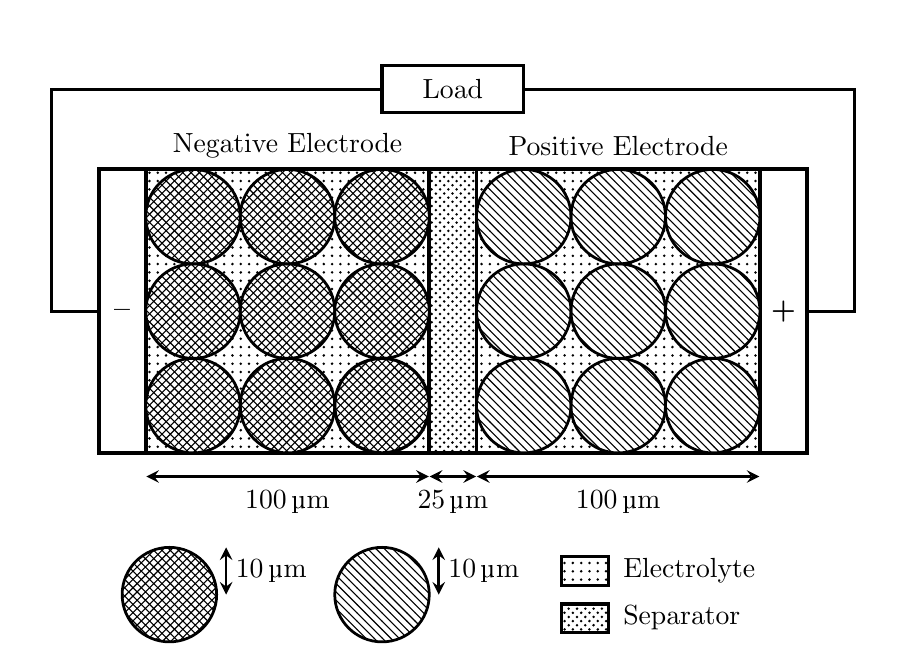
\begin{tikzpicture}[scale=0.6,>=stealth]
    	
        \draw[line width=0.4mm] (-7.5,0) -- (-8.5,0) --(-8.5,4.7)-- (8.5,4.7) -- (8.5,0) -- (7.5,0);
         \draw[line width=0.4mm, fill=white] (-1.5,4.2) rectangle (1.5,5.2);
         \node at (0,4.7){Load};
    	
		\draw[step=1cm,gray,very thin, draw=none] (-9,-7) grid (9,6);
        
        % Electrolyte
        \draw[line width=0.5mm, pattern=dots] (-6.5,-3) rectangle (6.5,3);
        
        % separator
        \draw[fill=white]  (-0.5,-3) rectangle (0.5,3);
        \draw[line width=0.5mm,pattern=crosshatch dots]  (-0.5,-3) rectangle (0.5,3);
        
        % Negative Current Collector
        \draw[line width=0.5mm] (-7.5,-3) rectangle (-6.5,3);
        
        % Positive Current Collector
        \draw[line width=0.5mm] (6.5,-3) rectangle (7.5,3);
        
        % negative electrode       
        \draw[fill=white,draw=none] (-5.5, 2) circle (1cm);
        \draw[fill=white,draw=none] (-5.5, 0) circle (1cm);
        \draw[fill=white,draw=none] (-5.5, -2) circle (1cm);        
        
        \draw[fill=white,draw=none] (-3.5, 2) circle (1cm);
        \draw[fill=white,draw=none] (-3.5, 0) circle (1cm);
        \draw[fill=white,draw=none] (-3.5, -2) circle (1cm);       
        
        \draw[fill=white,draw=none] (-1.5, 2) circle (1cm);
        \draw[fill=white,draw=none] (-1.5, 0) circle (1cm);
        \draw[fill=white,draw=none] (-1.5, -2) circle (1cm);
        
        
        
        \draw[line width=0.35mm,pattern=crosshatch, pattern color = black] (-5.5, 2) circle (1cm);
        \draw[line width=0.35mm,pattern=crosshatch, pattern color=black] (-5.5, 0) circle (1cm);
        \draw[line width=0.35mm,pattern=crosshatch, pattern color=black] (-5.5, -2) circle (1cm);        
        
        \draw[line width=0.35mm,pattern=crosshatch, pattern color=black] (-3.5, 2) circle (1cm);
        \draw[line width=0.35mm,pattern=crosshatch, pattern color=black] (-3.5, 0) circle (1cm);
        \draw[line width=0.35mm, pattern=crosshatch, pattern color=black] (-3.5, -2) circle (1cm);       
        
        \draw[ line width=0.35mm,pattern=crosshatch, pattern color=black] (-1.5, 2) circle (1cm);
        \draw[ line width=0.35mm,pattern=crosshatch, pattern color=black] (-1.5, 0) circle (1cm);
        \draw[ line width=0.4mm,pattern=crosshatch, pattern color=black] (-1.5, -2) circle (1cm);
        
        % positive electrode
        \draw[fill=white,draw=none] (1.5,2) circle (1cm);
        \draw[fill=white,draw=none] (1.5,0) circle (1cm);
        \draw[fill=white,draw=none] (1.5,-2) circle (1cm);
        
        \draw[fill=white,draw=none] (3.5,2) circle (1cm);
        \draw[fill=white,draw=none] (3.5,0) circle (1cm);
        \draw[fill=white,draw=none] (3.5,-2) circle (1cm);
        
        \draw[fill=white,draw=none] (5.5,2) circle (1cm);
        \draw[fill=white,draw=none] (5.5,0) circle (1cm);
        \draw[fill=white,draw=none] (5.5,-2) circle (1cm);
        
		\draw[line width=0.35mm,pattern=north west lines] (1.5,2) circle (1cm);
        \draw[line width=0.35mm,pattern=north west lines] (1.5,0) circle (1cm);
        \draw[line width=0.35mm,pattern=north west lines] (1.5,-2) circle (1cm);
        
        \draw[line width=0.35mm,pattern=north west lines] (3.5,2) circle (1cm);
        \draw[line width=0.35mm,pattern=north west lines] (3.5,0) circle (1cm);
        \draw[line width=0.35mm,pattern=north west lines] (3.5,-2) circle (1cm);
        
        \draw[line width=0.35mm,pattern=north west lines] (5.5,2) circle (1cm);
        \draw[line width=0.35mm,pattern=north west lines] (5.5,0) circle (1cm);
        \draw[line width=0.35mm,pattern=north west lines] (5.5,-2) circle (1cm);
      	
        % Sizes 
        %\draw[line width=0.35mm,<->] (-7.5,-3.5) -- (-6.51,-3.5);
        %\node[below] at (-7,-3.6) {$\SI{25}{\micro\metre}$};
        
        \draw[line width=0.35mm,<->] (-6.49,-3.5) -- (-0.51,-3.5);
        \node[below] at (-3.5,-3.6) {$\SI{100}{\micro\metre}$};
        
        \draw[line width=0.35mm,<->] (-0.49,-3.5) -- (0.49,-3.5);
        \node[below] at (0,-3.6) {$\SI{25}{\micro\metre}$};
        
        \draw[line width=0.35mm,<->] (0.51,-3.5) -- (6.49,-3.5);
        \node[below] at (3.5,-3.6) {$\SI{100}{\micro\metre}$};
        
        %\draw[line width=0.35mm,<->] (6.51,-3.5) -- (7.5,-3.5);
        %\node[below] at (7,-3.6) {$\SI{25}{\micro\metre}$};
        
        %% Bottom Box
        
        %\draw[line width=0.4mm] (-7.5,-7.2) rectangle (7.5,-4.8);
        
        \draw[line width=0.35mm,pattern=crosshatch, pattern color = black] (-6, -6) circle (1cm);
        \draw[line width=0.35mm,<->] (-4.8,-6) -- (-4.8,-5);
        \node[right] at (-4.8,-5.5){$\SI{10}{\micro\metre}$};
        
         \draw[line width=0.35mm,pattern=north west lines, pattern color = black] (-1.5, -6) circle (1cm);
        \draw[line width=0.35mm,<->] (-0.3,-6) -- (-0.3,-5);
        \node[right] at (-0.3,-5.5){$\SI{10}{\micro\metre}$};
              
        
        \draw[line width=0.35mm, pattern=dots] (2.3,-5.8) rectangle (3.3,-5.2);
        \node[right] at (3.4,-5.5){Electrolyte};
        
        \draw[line width=0.4mm, pattern=crosshatch dots] (2.3,-6.8) rectangle (3.3,-6.2);
        \node[right] at (3.4,-6.5){Separator};
        
         % Labels
        \node at (-7,0){{\bf --}};
        \node at (-3.5,3.5){Negative Electrode};
        \node at (3.5,3.5){Positive Electrode};
        
        %\node at (0,3.5){Separator};
        
        \node at (7,0){{\bf +}};
        
	\end{tikzpicture}
}

\newcommand{\voltage}{
	\centering
	\begin{tikzpicture}
	
			\begin{axis}
				[
				width=\textwidth,
				height=0.6\textwidth,
				xlabel={Discharge Capacity ($\SI{}{\ampere\hour/\metre^2}$)},
				ylabel={Voltage (V)},
				xmin=0,
  				xmax=25,
  				ymin=3.2,
  				ymax=3.9,  	
  				minor tick num=1,
  				grid=major, %both, major or minor
  				major grid style={dashed, line width=.1pt},
  				cycle list name=mylist, 
  				legend pos=outer north east,
  				legend style={name=leg}
				]	
				\foreach \x in {0.1, 0.5, 1, 2, 3}{
					\addplot table [col sep=comma, x index=0, y index=1]
					{plot/C\x.dat};
					
					\edef\temp{\noexpand\addlegendentry{\x C}}
					\temp
				}
				\foreach \x in {0.1, 0.5, 1, 2, 3}{
					\addplot table [col sep=comma, x index=0, y index=2]
					{plot/C\x.dat};
					\addplot table [col sep=comma, x index=0, y index=3]
					{plot/C\x.dat};
					}
			\end{axis}
							
			%\node[fill=white, draw, align=center, below=1mm, anchor=north east] (1) at (leg.south east) {Word: Text};
			
			\begin{customlegend}[legend entries={DFN,SPM,SPMe},legend style={at={(leg.south)},below=1mm, anchor=north}]
    			\addlegendimage{black, thick}
    			\addlegendimage{black,dashed, thick}
    			\addlegendimage{black, dotted, thick}
    		\end{customlegend}
	
	\end{tikzpicture}
}


\newcommand{\transient}{
	\begin{center} 
	\begin{tikzpicture}
	
			\begin{axis}
				[
				width=0.9\textwidth,
				height=0.5\textheight,
				xlabel={Discharge Capacity ($\SI{}{\ampere\hour/\metre^2}$)},
				ylabel={Voltage (V)},
				xmin=0,
  				xmax=1.5,
  				ymin=3.72,
  				ymax=3.78,  	
  				minor tick num=1,
  				grid=major, %both, major or minor
  				major grid style={dashed, line width=.1pt},
  				legend pos=north east,
  				legend style={name=leg}
				]	
				{
				\addplot[c1,thick] table [col sep=comma, x index=0, y index=1]
					{plot/voltage/transient1C.dat};
				\addplot[c2,thick, dashed] table [col sep=comma, x index=0, y index=2]
					{plot/voltage/transient1C.dat};
				\addplot[c3,thick, dashed] table [col sep=comma, x index=0, y index=3]
					{plot/voltage/transient1C.dat};
					
					\edef\temp{\noexpand\addlegendentry{DFN}}
					\temp
					\edef\temp{\noexpand\addlegendentry{SPMe}}
					\temp
					\edef\temp{\noexpand\addlegendentry{SPMeT}}
					\temp
				}
			\end{axis}						
	
	\end{tikzpicture}
	\end{center} 
}

\newcommand{\fastDischarge}{
	\begin{center} 
	\begin{tikzpicture}
	
			\begin{semilogyaxis}
				[
				width=0.8\textwidth,
				height=0.8\textheight,
				xlabel={$\hat{\lambda}$},
				ylabel={},
				xmin=1,
  				xmax=70,
  				ymin=1e-12,
  				ymax=1,  	
  				minor tick num=1,
  				grid=major, %both, major or minor
  				major grid style={dashed, line width=.1pt},
  				legend pos=north east,
  				legend style={name=leg}
				]	
				{
				\addplot[c1,thick] table [col sep=comma, x index=0, y index=1]
					{plot/SEI/fastDischargeLiError.csv};
				\addplot[c2,thick, dashed] table [col sep=comma, x index=0, y index=2]{plot/SEI/fastDischargeLiError.csv};
				\addplot[c3,thick] table [col sep=comma, x index=0, y index=1]{plot/SEI/fastDischargeGrowthError.csv};
				\addplot[c5,thick, dashed] table [col sep=comma, x index=0, y index=2]{plot/SEI/fastDischargeGrowthError.csv};
					
					\edef\temp{\noexpand\addlegendentry{Abs($\Delta q^+$)}}
					\temp
					\edef\temp{\noexpand\addlegendentry{$\exp(-\lambda y_0)$}}
					\temp
					\edef\temp{\noexpand\addlegendentry{Abs($\Delta q^-$)}}
					\temp
					\edef\temp{\noexpand\addlegendentry{$\exp(-2\lambda y_0)$}}
					\temp
				}
			\end{semilogyaxis}						
	
	\end{tikzpicture}
	\end{center} 
}

\newcommand{\fastCharge}{
	\begin{center} 
	\begin{tikzpicture}
	
			\begin{axis}
				[
				width=0.8\textwidth,
				height=0.8\textheight,
				xlabel={$\hat{\lambda}$},
				ylabel={Growth rate ($q^-$)}, 
				xmin=0,
  				xmax=200,
  				ymin=-5,
  				ymax=300,  	
  				minor tick num=1,
  				grid=major, %both, major or minor
  				major grid style={dashed, line width=.1pt},
  				legend pos=north west,
  				legend style={name=leg}
				]	
				{
				\addplot[c1,thick] table [col sep=comma, x index=0, y index=1]
					{plot/SEI/fastCharge.csv};
				\addplot[c2,thick, dashed] table [col sep=comma, x index=0, y index=2]{plot/SEI/fastCharge.csv};
					
					\edef\temp{\noexpand\addlegendentry{Numerical}}
					\temp
					\edef\temp{\noexpand\addlegendentry{Analytical}}
					\temp
				}
			\end{axis}						
	\end{tikzpicture}
	\end{center} 
}


 % for tikz and pgfplots code (this just keeps things in the main file clean)

\begin{document}

\begin{frontmatter}


\title{An Extended Single Particle Model with Electrolyte}
%\title{Elsevier \LaTeX\ template\tnoteref{mytitlenote}}
\tnotetext[mytitlenote]{Fully documented templates are available in the elsarticle package on \href{http://www.ctan.org/tex-archive/macros/latex/contrib/elsarticle}{CTAN}.}

%% Group authors per affiliation:
\author{Scott Marquis\fnref{oxford}, Valentin Sulzer\fnref{oxford}, Jon Chapman, Colin Please}
\address{University of Oxford}
\fntext[oxford]{Oxford}

%% or include affiliations in footnotes:
\author[mymainaddress,mysecondaryaddress]{Elsevier Inc}
\ead[url]{www.elsevier.com}

\author[mysecondaryaddress]{Global Customer Service\corref{mycorrespondingauthor}}
\cortext[mycorrespondingauthor]{Corresponding author}
\ead{support@elsevier.com}

\address[mymainaddress]{1600 John F Kennedy Boulevard, Philadelphia}
\address[mysecondaryaddress]{360 Park Avenue South, New York}

\begin{abstract}
This template helps you to create a properly formatted \LaTeX\ manuscript.
\end{abstract}

\begin{keyword}
\texttt{elsarticle.cls}\sep \LaTeX\sep Elsevier \sep template
\MSC[2010] 00-01\sep  99-00
\end{keyword}

\end{frontmatter}

\linenumbers

\section{Introduction} 
\subsection{Background}
Lithium-ion batteries are used extensively in consumer electronics and industry. In the management and design of batteries for these many applications, mathematical models are an essential tool. The standard mathematical model for a lithium-ion battery is the Doyle-Fuller Newman (DFN) model, which was developed by John Newman and cooperators in 1990s \cite{doyle,Fuller1994,newman_book}. However, for many applications, this model is overly complex. Instead, simpler models such as the Single Particle Model (SPM) are commonly employed within the control community \cite{Moura2017} (and others). \\

There have been several previous attempts to derive the SPM and various extensions (ciiite). However, these approaches generally rely on a number of unnecessary assumptions. In this work, we provide a rigorous mathematical derivation of the SPM and extensions by employing asymptotic methods. Similar methods have been used in the derivation of reduced models of lead acid batteries \cite{tino}. With our approach, we require only two assumptions: fast electrical conductivity in the negative and positive electrodes, and fast diffusion in the electrolyte. The validity of both of these assumptions is determined directly from the inputed parameter values. In comparison, six assumptions that can only be validated by comparison with the full DFN model are required in \cite{Moura2017}. Furthermore, our approach provides information regarding the accuracy of the reduced models. A key result of our work is a purely algebraic correction term which predicts the terminal voltage to a higher degree of accuracy than the SPM but with negligible additional computational requirements. 

\subsection{How a Lithium-ion Battery Works}
Lithium-ion batteries consist of two electrodes, a porous separator, an electrolyte, and two current collectors, as displayed in Figure \ref{fig:liBat}. We neglect the effects of the binder in this description. 
\begin{figure}[h!]
	\centering
	\LiBattery
    \caption{Schematic of a lithium-ion battery.}\label{fig:liBat}
\end{figure} 
Upon discharge, lithium intercalated in the negative electrode particles diffuses to the surface of the particles where a chemical reaction occurs. This chemical reaction produces a lithium ion free to move through the electrolyte and an electron free to move through the electrode. The electron travels through the electrode, into the current collector, through an external wire, and towards the positive electrode. Meanwhile, the lithium ion diffuses through the electrolyte towards the positive electrode. At the surface of the positive electrode particles, the lithium ion and the electron combine through another chemical reaction to form a lithium atom intercalated in the positive electrode particle. To charge, a voltage is applied across the cell and the whole process occurs in reverse.

\section{Derivation of Simplified Models}
\subsection{Doyle-Fuller-Newman Model}
We summarize here the 1+1D Doyle-Fuller-Newman (DFN) model which is the standard model of a lithium ion battery \cite{doyle,Fuller1994,newman_book}. The model is derived either by volume averaging (\cite{newman_book,Plett2004}) or the method of multiple scales \cite{Richardson2011}. In Appendix (NAME), we have address a recent concern from within the mathematical community related to the derivation of this model \cite{moyles2018asymptotic}. We denote quantities in the negative electrode, separator, and positive electrode regions with the subscript $k=n,s,p$, respectively. We also denote all dimensional quantities with a superscript $*$. A full list of the of the variables and dimensional parameters in the model can be found in Table (make) and Table \ref{tab:dimensional}, respectively. The full system of governing equations is summarized as: 
\begin{subequations} 	
    \begin{gather}
    	\epsilon_k \pdv{c_e^*}{t^*} = \pdv{x^*}\left(\epsilon_k^b D_e^*(c_e^*) \pdv{c_e^*}{x^*}\right) + a_k (1-t^+) G_k^*, \\ 
    	\pdv{i_e^*}{x^*} = a_k^* F^* G_k^*, \\ 
        i_e^* = \epsilon_k^b \kappa_e^*(c_e^*) \left( - \pdv{\phi_e^*}{x^*} + 2(1-t^+)\frac{R^*T^*}{F^*} \pdv{x^*}\left(\log(c_e^*)\right)\right)
    \end{gather} 

	\begin{gather}
     \pdv{c_k^*}{t^*} = \frac{1}{(r^*)^2}\pdv{r^*}\left((r^*)^2 D_k^*\pdv{c_k^*}{r^*}\right), \\
     \pdv{c_k^*}{r^*}\big|_{r^*=0} = 0, \ \ - D^*_k\pdv{c_k^*}{r^*}\big|_{r^*=R_k} = G_k^* \\
     i_k^* = -\kappa_k^* \pdv{\phi_k^*}{x^*}, \\ 
        \pdv{i_k^* }{x^*} = - a_s^* F^* G_k^* 
    \end{gather} 
 
    \begin{gather} 
    	G_k^* = \frac{m_k^*}{F^*} (c_k^*)^{1/2} (c_{k,\text{max}}^*-c_k^*)^{1/2}(c_e^*)^{1/2} \sinh\left(\frac{F^*\eta^*_k}{2R^*T^*} \right)\big|_{r^*=R_k^*}, \\ \eta^*_k = \phi_k^* - \phi_e^* - U_s^*(c_k^*),
    \end{gather} 
with the boundary conditions
    \begin{gather} 
    	\pdv{c_k^*}{x^*}\big|_{x^*=0,L^*}=0, \\ i_e^*\big|_{x^*=0,L^*}=0, \quad i_e^*\big|_{x^*=L_n^*,L^*-L_p^*}=I^*
    \end{gather} 
and initial conditions
    \begin{gather} 
    	c_k^*(x^*,r^*,0) = c_{k,0}^*, \quad c_e^*(x^*,0) = c^*_{e,\text{ref}}, \\ 
        \phi^*_{e}(x^*,0) = \phi^*_{e,0}, \quad \phi^*_{k}(x^*,0) = \phi^*_{k,0}.
    \end{gather} 
\end{subequations}
We prescribe functional forms taken from Newman's Dualfoil code for $U_n^*(c_n^*)$, $U_p^*(c_p^*)$, and $D_e^*(c_e^*)$, which are the open circuit potentials (OCP) at the negative and positive electrodes and the lithium ion diffusivity in the electrolyte, respectively \cite{newman2004fortran}. These can be found in Appendix \ref{app:paraFun}. This correspond to a cell with a graphite negative electrode, an \ce{LiPF6} in EC:DMC electrolyte, and a lithium cobalt oxide positive electrode. We note here, that we (as is done by Newman) have taken lithium diffusivity in the solid to be concentration independent but that this does not effect the derivation of our simplified models. 

\subsection{Dimensionless Form of DFN model}
We use asymptotic methods to reduce the DFN model to a number of simpler forms. To do this, we first nondimensionalise the DFN model by making the following scalings: 
\begin{gather}	
	\begin{split}
	r^* = R_s^* r_s, \quad x^* = L^* x, \quad t^* = \tau_d^* t \\ 
    c_n^* = c_{n,\text{max}}^*c_n, \quad c_e^* = c_{e,\text{ref}} c_e, \quad c_p^* = c_{p,\text{max}}^* c_p, \\
    \phi_n^* = \Phi^* \phi_n, \quad \phi_e^* = \Phi^* \phi_e, \quad \phi_p^*=\Phi^* \phi_p, \\ 
    U_n^*(c_n^*) = \Phi^* U_n(c_n) \quad U_p^*(c_p^*) = \Phi^* U_p(c_p) \\
    i_n^*= J^* i_n, \quad i_e^* = J^* i_e, \quad i_p^* = J^* i_p, \\ 
    G_n^* = \frac{J^*}{a_n^* F^* L^*}G_n, \quad G_p^* = \frac{J^*}{a_p^* F^* L^*}G_p, \\ 
    D_e^*(c_e^*) = \tilde{D}_e^* D_e(c_e) \quad 
    \kappa^*_e(c_e^*) = \frac{(F^*)^2 \tilde{D}_e^* c_{e,\text{ref}}^*}{R^*T^*}\kappa(c_e)
    \end{split}
\end{gather} 
and identify the following timescales in the model: 
\begin{gather} 
	\begin{split}
	\tau_d^*=\frac{F^* c_{n,\text{max}}^* L^*}{J^*},\quad \tau_n^* = \frac{(R_n^*)^2}{D_n^*}, \quad \tau_e^* = \frac{(L^*)^2}{\tilde{D}_e^*}, \\ \tau_p^* = \frac{(R_p^*)^2}{D_p^*}, \quad \tau_{r_n}^* = \frac{F^*}{m_n^* a_n^* (c_{e,\text{ref}}^*)^{1/2}}, \quad \tau_{r_p}^* = \frac{F^*}{m_p^* a_p^* (c_{e,\text{ref}}^*)^{1/2}},
    \end{split}
\end{gather} 
which correspond to the discharge timescale, the negative electrode diffusion timescale, electrolyte diffusion timescale, the positive electrode diffusion timescale, the negative electrode reaction timescale, and the positive electrode reaction timescale, respectively. We then identify the following dimensionless parameters
\begin{gather} 
	\begin{split}
	\gamma_n = \frac{\tau_d^*}{\tau_n^*}, \quad \gamma_p = \frac{\tau_d^*}{\tau_p^*}, \quad \beta_n = a_n^*R_n^*, \quad \beta_p = a_p^*R_p^*, \\ 
    \kappa_n = \frac{\kappa_n^* \Phi^*}{J^* L^*}, \quad \kappa_p = \frac{\kappa_p^* \Phi^*}{J^* L^*}, \quad m_n =\frac{\tau_d^*}{\tau_{r_n}^*}, \quad m_p =\frac{\tau_d^*}{\tau_{r_p}^*}, \\ 
    \hat{C}_k=\frac{c_{k,\text{max}}^*}{c_{n,\text{max}}^*}, \quad \nu=\frac{c_{n,\text{max}}^*}{c_{e,\text{ref}}^*}, \quad \lambda=\frac{F^* \Phi^*}{R^* T^*}, \quad \delta = \frac{\tau_e^*}{\tau_{d}^*}.
    \end{split}
\end{gather}
The values of these dimensionless parameters are given in Table \ref{tab:nonDim} in terms of the C-rate for the dimensional parameters in Table \ref{tab:dimensional}. The resulting dimensionless equations are summarized as: 

\begin{subequations}\label{eqn:DFN} 	
	
     \begin{gather} 
    	\delta \epsilon_k \pdv{c_e}{t} = \epsilon_k^b \pdv{x}\left(D_e(c_e) \pdv{c_e}{x}\right) + \delta \nu (1-t^+) G_k \label{eqn:nDim:electrolyte:concentration}\\
    	\pdv{i_e}{x} = G_k, \label{eqn:nDim:electrolyte:current} \\ 
        \delta \nu i_e = \kappa(c_e) \left( -\lambda \pdv{\phi_e}{x} + 2(1-t^+) \pdv{x}\left(\log(c_e)\right)\right)\label{eqn:nDim:McIn}
    \end{gather} 
    
	\begin{gather}
     \pdv{c_k}{t} = \gamma_k \frac{1}{r_k^2}\pdv{r_k}\left(r_k^2 \pdv{c_k}{r_k}\right), \label{eqn:nDim:solid:concentration} \\
     \pdv{c_k}{r}\big|_{r_k=0} = 0, \ \ - \beta_k \hat{C}_k \gamma_k  \pdv{c_k}{r_k}\big|_{r_k=1} = G_k \label{eqn:nDim:solid:con:BC} \\
    	\pdv{i_k}{x} = - G_k \label{eqn:nDim:solid:current}\\  
        i_k = - \kappa_k \pdv{\phi_k}{x}, \label{eqn:nDim:solid:ohms}
    \end{gather}    
 
    \begin{gather} 
    	G_k = m_k \hat{C}_k c_k^{1/2} (1-c_k)^{1/2}c_e^{1/2} \sinh\left(\frac{\lambda \eta_k}{2} \right)\big|_{r_s=1}, \\ \eta_k = \phi_k - \phi_e - U_k(c_k) \label{eqn:nDim:BV}
    \end{gather} 
    
with the boundary conditions: 
    
    \begin{gather}\label{eqn:nDim:BC}
    	\pdv{c_e}{x}\big|_{x=0,1}=0, \quad i_e\big|_{x=0,1}=0, \quad i_e\big|_{x=l_n,1-l_p}=I
    \end{gather}     
and initial conditions 
    \begin{gather}\label{eqn:nDim:init}
    	c_k(x,r,0) = c_{k,0}, \ \ c_e(x,0) = 1, \ \ \phi_{e}(x,0) = \phi_{e,0}, \ \ \phi_{s}(x,0) = \phi_{s,0}.
    \end{gather} 
\end{subequations}

\subsection{Leading Order Model (SPM)}
\scott{Need to work this carefully I think. Maybe say  typical C-rates (i.e 0.5C-5C) instead}
A key observation from Table \ref{tab:nonDim} is that for C-rates below 5C, we have that $1/\kappa_k \ll \delta^2 \ll \delta \ll 1$, whereas all other parameters are $\mathcal{O}(1)$. Therefore, we seek the following asymptotic expansions
\begin{align*} 
	&c_k \sim c_k^0 + \delta c_k^1 + \dots \ \ 
    &&c_k \sim c_k^0 + \delta c_k^1 + \dots \\ 
    &\phi_k \sim \phi_k^0 + \delta \phi_k^1 + \dots \ \ 
    &&\phi_e \sim \phi_e^0 + \delta \phi_e^1 + \dots \\
    &i_k \sim i_k^0 + \delta i_k^1 + \dots \ \ 
    &&i_e \sim i_e^0 + \delta i_e^1 + \dots \\    
     &G_k \sim G_k^0 + \delta G_k^1 + \dots 
\end{align*}
At leading order, (\ref{eqn:nDim:electrolyte:concentration}) gives
\begin{equation}
	\pdv{x}\left(\mathcal{D}_e(c_e^0) \pdv{c_e^0}{x}\right) = 0, 
\end{equation}
\scott{Derive the time independence of $c_e^0$}
which determines that $c_e^0$ is independent of $x$. Furthermore, we also have that $c_e^0=1$ from (\ref{eqn:nDim:init}) and the time independence of $c_e^0$ (WHICH COMES FROM...). Equation (\ref{eqn:nDim:McIn}) at leading order, then gives: 
\begin{equation}
	\pdv{\phi_e^0}{x} = 0 
\end{equation}
and so $\phi_e^0 = \phi_e^0(t)$. We now take advantage of the fact that $1/\kappa_k \ll \delta$, so that at leading order (\ref{eqn:nDim:solid:current}) gives 
\begin{equation}
	\pdv{\phi_k}{x} = 0 
\end{equation}
and hence $\phi_k = \phi_k(t)$.  
Since $c_k^0$ is initially independent of $x$ and $c_e^0$, $\phi_e^0$, and $\phi_k^0$ are all independent of $x$, it follows from (\ref{eqn:nDim:BV}) at leading order that $G_k^0$ and $c_k^0$ are independent of $x$ for all time. Therefore, we can integrate (\ref{eqn:nDim:electrolyte:current}) over electrode $k$ and apply (\ref{eqn:nDim:BC}) to find: 
\begin{gather} 
	i_e^0 = 
    \begin{cases} 
    \frac{x}{l_n}I, &0\leq x \leq l_n \\
    I, & l_n\leq x \leq 1-l_p \\
    \frac{1-x}{l_p}I, & l_p\leq x \leq 1
    \end{cases}
\end{gather} 
which determines $G_n^0=I(t)/l_n$ and $G_p^0=-I(t)/l_p$. Solving (\ref{eqn:nDim:BV}) at leading order gives
\begin{equation}\label{eqn:lo:phi}
	\phi_k^0 = \phi_e^0 + U_k(c_k^0) + \frac{2}{\lambda}\sinh^{-1}\left( \frac{G_k^0}{g_k^0} \right), \ \ \text{for} \ k\in\{n,p\}, 
\end{equation}
where 
\begin{equation}\label{eqn:gk0} 
g_k^0=m_k \hat{C}_k (c^0_k)^{1/2} (1-c_k^0)^{1/2}(c_e^0)^{1/2}.
\end{equation}
from which we can determine the leading order terminal voltage, $V^0=\phi_p^0-\phi_n^0$, is given by 
\begin{subequations}\label{eqn:SPM} 
\begin{align} 
	\begin{split}
	V^0(t) = &U_p(c_p^0) - U_n(c_n^0) - \frac{2}{\lambda}\sinh^{-1}\left( \frac{I(t)}{g_p^0 l_p} \right) - \frac{2}{\lambda} \sinh^{-1}\left( \frac{I(t)}{g_n^0 l_n} \right).
    \end{split} 
\end{align} 

Therefore, one must now only determine $c_k^0$ in order to determine the the leading order terminal voltage. At leading order (\ref{eqn:nDim:solid:concentration}) and (\ref{eqn:nDim:solid:con:BC}) give 
	\begin{align} \label{eqn:lo:solidConcentration} 
     \pdv{c_k^0}{t} = \gamma_k \frac{1}{r_k^2}\pdv{r_k}\left(r_k^2 \pdv{c_k^0}{r_k}\right), \\
     \pdv{c_k^0}{r}\big|_{r_k=0} = 0, \ \ - \beta_k\hat{C}_k \gamma_k \pdv{c_k^0}{r_k}\big|_{r_k=1} = G_k^0  \label{eqn:lo:solidConcentration:BC} 
    \end{align} 
\end{subequations} 
which is solved numerically. We identify (\ref{eqn:SPM}) as the dimensionless form of the commonly used single particle model (SPM) [Reference Howey and some other people using the SPM model]. \\

\subsection{Next Order Correction}
We now proceed to $\mathcal{O}(\delta)$ to extend the range of applicability of the SPM model to higher C-rates. At $\mathcal{O}(\delta)$, (\ref{eqn:nDim:electrolyte:concentration}) becomes
\begin{equation}\label{eqn:od:electrolyte} 
    	 \pdv{x}\left(\epsilon_k^b D_e(c^0_e) \pdv{c^1_e}{x}\right) + \nu (1-t^+) G_k^0 = 0. 
\end{equation} 
With the conditions of continuity of the flux and concentration of lithium at the electrode--separator boundaries given as
\begin{align}
	c_{e,n}=c_{e,s}, \quad \epsilon_n^b \pdv{c_{e,n}^1}{x} = \epsilon_s^b \pdv{c_{e,s}^1}{x}, \quad \text{on} \, x=l_n, \\
    c_{e,s}=c_{e,p}, \quad \epsilon_s^b \pdv{c_{e,s}^1}{x} = \epsilon_p^b \pdv{c_{e,p}^1}{x}, \quad \text{on} \, x=1-l_p,
\end{align}
where $c_{e,k}$ is the electrolyte concentration in region $k$, we integrate (\ref{eqn:od:electrolyte}) over the entire cell and apply the leading order boundary conditions from (\ref{eqn:nDim:BC}), to find: 
\begin{align} 
	\begin{split}
	c_e^1(x,t) =&\frac{\nu (1-t^+) I(t)}{ 6 \mathcal{D}(c_e^0)}\left( 2\left(\frac{l_p^2}{\epsilon_p^b} - \frac{l_n^2}{\epsilon_n^b}\right) + 3\begin{cases} 
    	  \frac{l_{sep}}{\epsilon_{sep}^b}(1+l_p-l_n) + \frac{1}{\epsilon_n^b l_n}(l_n^2-x^2) , & 0\leq x \leq l_n \\
    	  \frac{1}{\epsilon_{sep}^b}(l_n^2 - l_p^2 + 1-2x) , & l_n\leq x \leq 1-l_p \\
    	  \frac{l_{sep}}{\epsilon_{sep}^b}(l_p - l_n - 1) + \frac{1}{l_p \epsilon_p^b}( (x-1)^2 - l_p^2 ), & 1-l_p\leq x \leq 1
    \end{cases}  \right) 
    \end{split}
\end{align} 
\scott{Probably need to split this in some way}
At $\mathcal{O}(\delta)$, (\ref{eqn:nDim:McIn}) becomes
\begin{gather} 
        \nu i_e^0 = \epsilon_k^b \kappa(c_e^0) \left( -\lambda \pdv{\phi^1_e}{x} + \frac{2(1-t^+)}{c_e^0} \pdv{c_e^1}{x} \right)
\end{gather} 
Integration in $x$ and application of the continuity conditions at $x=l_n$ and $x=1-l_p$ (we note that the flux conditions are already automatically satisfied), gives
\begin{equation} 
	\phi_e^1(x,t) =\tilde{\phi}_e^1(t) + \frac{2(1-t^+)}{\lambda c_e^0}c_e^1 - \frac{\nu I(t)}{\lambda \kappa(c_e^0)}
    \begin{cases} 
    	   \frac{x^2-l_n^2}{2 \epsilon_n^b l_n} + \frac{l_n}{\epsilon_{sep}^b}, & 0\leq x \leq l_n \\
    	   \frac{x}{\epsilon_{sep}^b}, & l_n\leq x \leq 1-l_p \\
    	   \frac{x(2-x)+l_p^2-1}{2\epsilon_p^b l_p} + \frac{1-l_p}{\epsilon_{sep}^b}, & 1-l_p\leq x \leq 1
    \end{cases}  
\end{equation} 
where we $\tilde{\phi}_e^1(t)$ is determined by an arbitrarily chosen ground potential. \\

At $\mathcal{O}(\delta)$ (\ref{eqn:nDim:electrolyte:current}) and (\ref{eqn:nDim:BC}) become
\begin{align}\label{eqn:od:elect:curr}
	\pdv{i_e^1}{x} = G_k^1, \quad i_e^1\bigg|_{x=0,l_n,1-l_p,1} = 0 
\end{align} 
Integration of (\ref{eqn:od:elect:curr}) over each electrode separately then gives the conditions
\begin{equation}\label{eqn:od:conditions} 
	\int_0^{l_n} G_n^1(x,t)\, \text{d}x = 0, \ \ \int_{1-l_p}^1 G_p^1(x,t)\, \text{d}x = 0. 
\end{equation}
The $\mathcal{O}(\delta)$ component of (\ref{eqn:nDim:BV}) is given by
    \begin{gather} \label{eqn:od:BV}
    	G_k^1 = \frac{g_k^0}{2} \left( g_k^1 \sinh\left( \frac{\lambda\eta_k^0}{2}  \right) + \cosh(\frac{\lambda\eta_k^0}{2} ) \lambda \eta_k^1 \right)\bigg|_{r_k=1}, \\ \eta_k^0 = \phi^0_k - \phi^0_e - U_s(c_k), \ \ \eta_k^1 = \phi^1_k - \phi^1_e - U_k'(c^0_k)c_k^1\\
    g_k^1 = \left(\frac{c_k^1}{c_k^0} - \frac{c_k^1}{1-c_k^0} + \frac{c_{e,k}^1}{c_e^0} \right) 
    \end{gather} 
where $g_k^0$ is given by (\ref{eqn:gk0}). Given that $1/\kappa_k\ll\delta$, (\ref{eqn:nDim:solid:current}) at $\mathcal{O}(\delta)$ yields $\phi_k^1$ independent of $x$. We now average (\ref{eqn:od:BV}) over electrode $k$, apply the conditions in (\ref{eqn:od:conditions}), and rearrange for $\phi_k^0$ to find:
\begin{gather}\label{eqn:od:BV_av}
	\phi_s^1 = \bar{\phi}_{e,s}^1 + U_s'(c_s^0)\bar{c}_s^1 - \frac{\bar{g}_s^1G_s^0}{\lambda\sqrt{(g_s^0)^2 + (G_s^0)^2}}, \ \ s\in\{n,p\}
\end{gather} 
where we have used that
\begin{equation} 
	\tanh\left(\sinh^{-1}\left(\frac{G_s^0}{g_s^0} \right) \right) = \frac{G_s^0}{\sqrt{(g_s^0)^2 + (G_s^0)^2}}.
\end{equation}
and the averaged quantities are found from 
\begin{equation*}
	\bar{y}_n = \frac{1}{l_n}\int_{0}^{l_n}y_n\, \text{d}x, \quad 		\bar{y}_p = \frac{1}{l_p}\int_{0}^{l_p}y_p\, \text{d}x.
\end{equation*}
Upon calculation, these are given by 
\begin{align} 	
	\bar{c}_{e,n}^1 &= \frac{\nu (1-t^+) I(t)}{ 6 \mathcal{D}(c_e^0)}\left( 2\left(\frac{l_p^2}{\epsilon_p^b} - \frac{l_n^2}{\epsilon_n^b} \right) + \frac{2 l_n}{\epsilon_n^b} + \frac{3l_{sep}}{\epsilon_{sep}^{b}}(l_p-l_n+1)\right) \\ 
    \bar{c}_{e,p}^1 &= \frac{\nu (1-t^+) I(t)}{ 6 \mathcal{D}(c_e^0)}\left( 2\left(\frac{l_p^2}{\epsilon_p^b} - \frac{l_n^2}{\epsilon_n^b} \right) - \frac{2 l_p}{\epsilon_p^b} + \frac{3l_{sep}}{\epsilon_{sep}^{b}}(l_p-l_n-1)\right) \\ 
    \bar{\phi}_{e,n}^1 &= \tilde{\phi}_e^1(t) +\frac{2(1-t^+)}{\lambda c_e^0} \bar{c}_{e,n}^1 + \frac{\nu I(t)l_n}{\lambda \kappa(c_e^0)}\left(\frac{1}{3 \epsilon_{n}^b} - \frac{1}{\epsilon_{sep}^b}\right) \\ 
    \bar{\phi}_{e,p}^1 &= \tilde{\phi}_e^1(t) +\frac{2(1-t^+)}{\lambda c_e^0} \bar{c}_{e,p}^1 + \frac{\nu I(t)l_p}{\lambda \kappa(c_e^0)}\left(\frac{1}{ \epsilon_{sep}^b} - \frac{1}{3\epsilon_p^b}\right) - \frac{\nu I(t)}{\lambda \kappa(c_e^0)\epsilon_{sep}^b} \\
    \bar{g}_k^1 =& \left(\frac{\bar{c}_k^1}{c_k^0} - \frac{\bar{c}_k^1}{1-c_k^0} + \frac{\bar{c}_{e,k}^1}{c_e^0} \right).
\end{align} 
Taking the $O(\delta)$ component of (\ref{eqn:nDim:solid:concentration}) and (\ref{eqn:nDim:solid:con:BC}) and averaging over the electrode gives the following problem for $\bar{c}_k$: 
\begin{gather}
     \pdv{\bar{c}_k^1}{t} = \gamma_k \frac{1}{r_k^2}\pdv{r_k}\left(r_k^2 \pdv{\bar{c}_k^1}{r_s}\right), \\
     \pdv{\bar{c}_s^1}{r}\big|_{r_s=0} = 0, \\ 
     \left(\pdv{\bar{c}_s^1}{r_s}\right)\bigg|_{r_s=1} = 0.
    \end{gather} 
With the initial condition of $\bar{c}_k^1=0$ from $\mathcal{\delta}$ of (\ref{eqn:nDim:init}), we then must have ${\bar{c}_k^1=0}$ for all time (this also holds for non constant diffusivity). Therefore, our next order correction to the terminal voltage, ${V^1=\phi_p^1-\phi_n^1}$, is given by
\begin{align}\label{eqn:voltageCorrection}
\begin{split} 
V^1(t) = &-\frac{2 \nu (1-t^+)^2I(t)}{\lambda \mathcal{D}(c_e^0)c_e^0}\left( \frac{l_n}{3 \epsilon_n^b} + \frac{l_{sep}}{\epsilon_{sep}^b} + \frac{l_p}{3\epsilon_p^b} \right) \\ 
    & - \frac{\nu I(t)}{\lambda \kappa(c_e^0)} \left(\frac{l_n}{3\epsilon_n^b} - \frac{l_n - 1 + l_p}{\epsilon_{sep}^b} + \frac{l_p}{3\epsilon_p^b} \right) \\
    &+ \frac{\bar{g}_p^1 I(t) }{\lambda \sqrt{(g_p^0l_p)^2+I(t)^2}} + \frac{\bar{g}_n^1 I(t) }{\lambda \sqrt{(g_n^0l_n)^2+I(t)^2}}.  
\end{split}
\end{align} 
With the correction term our terminal voltage is now given by $V=V^0+\delta V^1$ which is now $\mathcal{O}(\delta^2,1/\kappa_p)$ accurate instead of just $\mathcal{O}(\delta)$ accurate in the case of the SPM. Therefore, this model increases the accuracy of the SPM with the only addition being a purely algebraic expression. 

\subsection{A simplified expression} 
In order to simplify the final form of the SPMe and to aid with interpretation, we note that
\begin{align*} 
	&-\frac{2}{\lambda}\sinh^{-1}\left(\frac{I}{\bar{g}_k l_k}\right) = -\frac{2}{\lambda}\sinh^{-1}\left(\frac{I}{g_k^0l_k} \right)
    +\delta \frac{\bar{g}_k^1 I}{\lambda\sqrt{(g_k^0l_k)^2+I^2}} 
    + \mathcal{O}\left(\delta^2\right)
\end{align*} 
where 
\begin{equation} 
	\bar{g}_k = m_k  (c_k^0)^{1/2}(1-c_k^0)^{1/2}(c_e^0+\delta\bar{c}_{e,k}^1 )^{1/2}
\end{equation} 
(recalling that $\bar{c}_k=0$). Therefore, we can express the voltage predicted by the SPMe as: 
\begin{align}\label{eqn:simple}
\begin{split} 
V(t) &= U_p(c_p^0) - U_n(c_n^0) \\
	 & - \frac{2}{\lambda}\sinh^{-1}\left( \frac{I(t)}{\bar{g}_p l_p} \right) 
     - \frac{2}{\lambda} \sinh^{-1}\left( \frac{I(t)}{\bar{g}_n l_n} \right) \\ 
     &-\delta\frac{2 \nu (1-t^+)^2I(t)}{\lambda \mathcal{D}(c_e^0)c_e^0}\left( \frac{l_n}{3 \epsilon_n^b} + \frac{l_{sep}}{\epsilon_{sep}^b} + \frac{l_p}{3\epsilon_p^b} \right) \\ 
    & - \delta \frac{\nu I(t)}{\lambda \kappa(c_e^0)} \left(\frac{l_n}{3\epsilon_n^b} - \frac{l_n - 1 + l_p}{\epsilon_{sep}^b} + \frac{l_p}{3\epsilon_p^b} \right)
\end{split}
\end{align} 
and retain $\mathcal{O}(\delta^2)$ accuracy. 

\subsection{An Extension for Solid Phase Ohmic Losses}
For the case $1/\kappa_k=\mathcal{O}(\delta)$, we include an additional term in the voltage to account for ohmic losses in the solid phase. We define $\tilde{\kappa}_k=\kappa_k \delta = \mathcal{O}(1)$ so that (\ref{eqn:nDim:solid:ohms}) becomes
\begin{equation} 
	\mathcal{\delta} i_k = -\tilde{\kappa}_k \pdv{\phi_k}{x} 
\end{equation} 
After making expansions in $\delta$, at leading order, we again obtain $\phi_k^0$ independent of $x$ and recover the SPM (\ref{eqn:SPM}). However, at $\mathcal{O}(\delta)$ we obtain 
\begin{equation} 
	\tilde{\kappa_k} \pdv{\phi_k^1}{x} = - i_k^0 = i_e^0-I =
    \begin{cases} 
    I(x/l_n - 1), \quad &0\leq x\leq l_n \\ 
    I((1-x)/l_p - 1), \quad &1-l_p \leq x \leq 1 
    \end{cases}
\end{equation} 
Therefore, we have 
\begin{align} 
	\phi_n^1 &= \tilde{\phi}_n^1 - \frac{I}{\tilde{\kappa}_n}\left(x - \frac{x^2}{2l_n}\right), \\ 
    \phi_p^1 &= \tilde{\phi}_p^1 - \frac{I}{l_p} \left( x - \frac{x}{l_p} + \frac{x^2}{2l_p} \right) 
\end{align} 
and 
\begin{align} 
\bar{\phi}_n^1 &= \frac{1}{l_n} \int_0^{l_n}\phi_n^1\, \text{d}x = \tilde{\phi}_n^1 - \frac{I l_n}{3 \tilde{\kappa}_n}, \\ 
\bar{\phi}_p^1 &= \frac{1}{l_p} \int_{1-l_p}^{1}\phi_p^1\, \text{d}x = \tilde{\phi}_p^1 + \frac{I}{6 \tilde{\kappa}_p l_p}\left(2l_p^2 - 6l_p + 3 \right).
\end{align}
Then (\ref{eqn:od:BV_av}) must be modified to 
\begin{gather}
	\bar{\phi}_k^1 = \bar{\phi}_{e,k}^1 + U_s'(c_k^0)\bar{c}_k^1 - \frac{\bar{g}_k^1G_k^0}{\lambda\sqrt{(g_k^0)^2 + (G_k^0)^2}}, \ \ k\in\{n,p\}
\end{gather} 
from which we determine (noting that $\bar{c}^1_k=0$)
\begin{align} 
	\tilde{\phi}_n^1 &= \bar{\phi}_{e,n}^1 +\frac{Il_n}{2\tilde{\kappa}_n} - \frac{\bar{g}_n^1I}{\lambda\sqrt{(g_n^0l_n)^2 + I^2}}, \\
    \tilde{\phi}_p^1 &= \bar{\phi}_{e,n}^1 - \frac{I}{6 \tilde{\kappa}_p l_p}\left(2l_p^2 - 6l_p + 3 \right) + \frac{\bar{g}_p^1I}{\lambda\sqrt{(g_p^0l_p)^2 + I^2}}.
\end{align} 
The new $\mathcal{O}(\delta)$ voltage is then given by

\begin{align}
 \begin{split} 
V^1(t) &= \phi_p(1) - \phi_n(0) \\ 
	&=-\frac{2 \nu (1-t^+)^2I(t)}{\lambda \mathcal{D}(c_e^0)c_e^0}\left( \frac{l_n}{3 \epsilon_n^b} + \frac{l_{sep}}{\epsilon_{sep}^b} + \frac{l_p}{3\epsilon_p^b} \right) \\ 
    & - \frac{\nu I(t)}{\lambda \kappa(c_e^0)} \left(\frac{l_n}{3\epsilon_n^b} - \frac{l_n - 1 + l_p}{\epsilon_{sep}^b} + \frac{l_p}{3\epsilon_p^b} \right) \\
    &+ \frac{\bar{g}_p^1 I(t) }{\lambda \sqrt{(g_p^0l_p)^2+I(t)^2}} + \frac{\bar{g}_n^1 I(t) }{\lambda \sqrt{(g_n^0l_n)^2+I(t)^2}} \\ 
    & - \frac{I}{3}\left(\frac{l_p}{\tilde{\kappa}_p}-\frac{l_n}{\tilde{\kappa}_n}\right) 
\end{split}
\end{align} 
where the first four terms remain the same as before and the final term represent the Ohmic losses in the solid phase. 
\section{Summary of SPMe in Dimensional Form}

\begin{subequations}
\begin{gather} 
     \pdv{c_k^*}{t^*} = \frac{1}{(r^*)^2}\pdv{r^*}\left((r^*)^2 D_k^* \pdv{c_k^*}{r^*}\right), \\
     \pdv{c_k^*}{r^*}\big|_{r^*=0} = 0, \quad - D_k^*\pdv{c_k^*}{r^*}\big|_{r^*=R_k^*} = 
     \begin{cases}
     I^*/(a_n^* F^* L_n), \quad \text{for} \ k=n\\ 
     -I^*/(a_p^* F^* L_p)\quad \text{for} \ k=p
     \end{cases}
\label{eqn:lo:solidConcentration:BC} 
\end{gather} 


\begin{align} 
	\begin{split} 
V^* &= U_p^*(c_p^{*}) - U_n^*(c_n^{*}) 
\\ &- \frac{2R^*T^*}{F^*}\sinh^{-1}\left(\frac{I^*}{F^*a_n^*L_n^* \bar{g}_n^{*}}\right) \\
&- \frac{2R^*T^*}{F^*}\sinh^{-1}\left(\frac{I^*}{F^*a_p^*L_p^* \bar{g}_p^{*}}\right) \\ 
&-\frac{R^* T^* (1-t^+)^2 I^*}{(F^*)^2 D_e^*(c_e^{*}) c_e^{*}}\left(\frac{L_n^*}{3\epsilon_n^b} + \frac{L_s^*}{\epsilon_s^b} + \frac{L_p}{3\epsilon_p^b} \right) \\ 
&-\frac{I^*}{\kappa^*(c_e^{*})}\left(\frac{L_n^*}{2\epsilon_n^b} - \frac{L_n^* - L^* + L_p^*}{\epsilon_s^b} + \frac{L_p^*}{2\epsilon_p^b} \right)
\end{split}
\end{align} 

where
\begin{align} 
	g_k^* &= \frac{m_k^*}{F^*} (c_k^*)^{1/2} (c^*_{k,\text{max}}-c_k^*)^{1/2}(c_e^* + \bar{c}_{e,k}^*)^{1/2}\bigg|_{r=R_k}, \quad \text{for} \ k=n,p \\	
	\bar{c}^*_{e,n} &= \frac{(1-t^+) I^*}{ 6 F^* D^*(c_e^*)}\left( 2\left(\frac{(L_p^*)^2}{L^*\epsilon_p^b} - \frac{(L_n^*)^2}{L^*\epsilon_n^b} \right) + \frac{2 L_n^*}{\epsilon_n} + \frac{3L^*_{s}}{L^*\epsilon_{s}^{b}}(L_p^*-L_n^*+L^*)\right) \\ 
    \bar{c}^*_{e,p} &= \frac{(1-t^+) I(t)}{ 6 F^* D^*(c_e^*)}\left( 2\left(\frac{(L_p^*)^2}{L^*\epsilon_p^b} - \frac{(L_n^*)^2}{L^*\epsilon_n^b} \right) - \frac{2 L_p^*}{\epsilon_p} + \frac{3L^*_{s}}{L^*\epsilon_{s}^{b}}(L^*_p-L^*_n-L^*)\right)
\end{align}
\end{subequations} 

Dimensional Voltage (note the superscript notation has been removed because it is too messy): 
\begin{align} 
	\begin{split} 
V^* = &U_p^*(c_p^{*}) - U_n^*(c_n^{*}) 
\\ &- \frac{2R^*T^*}{F^*}\sinh^{-1}\left(\frac{I^*}{F^*a_n^*L_n^* g_n^{*}}\right) \\
&- \frac{2R^*T^*}{F^*}\sinh^{-1}\left(\frac{I^*}{F^*a_p^*L_p^* g_p^{*}}\right) \\ 
&-\frac{R^* T^* (1-t^+)^2 I^*}{(F^*)^2 D_e^*(c_e^{*}) c_e^{*}}\left(\frac{L_n^*}{3\epsilon_n^b} + \frac{L_s^*}{\epsilon_s^b} + \frac{L_p}{3\epsilon_p^b} \right) \\ 
&-\frac{I^*}{\kappa^*(c_e^{*})}\left(\frac{L_n^*}{2\epsilon_n^b} - \frac{L_n^* - L^* + L_p^*}{\epsilon_s^b} + \frac{L_p^*}{2\epsilon_p^b} \right) \\ 
&+\frac{R^* T^*}{(F^*)^2}\frac{\bar{g}_n^* I^*}{\sqrt{(g_n^* F^* a_n^* L_n^*)^2+ (I^*)^2}} \\ 
&+\frac{R^* T^*}{(F^*)^2}\frac{\bar{g}_p^* I^*}{\sqrt{(g_p^* F^* a_p^* L_p^*)^2+ (I^*)^2}}
\end{split}
\end{align} 
where 
\begin{align} 
	g_k^* &= \frac{m_k^*}{F^*} (c_k^*)^{1/2} (c^*_{k,\text{max}}-c_k^*)^{1/2}(c_e^*)^{1/2}\bigg|_{r=R_k} \\
    \bar{g}_n^* &= \frac{(1-t^+)I^*}{6 c_e^* D_e^*(c_e^*)}\left( 2\left(\frac{(L_p^*)^2}{L^*\epsilon_p^b} - \frac{(L_n^*)^2}{L^*\epsilon_n^b} \right) + \frac{2 L_n^*}{\epsilon_n} + \frac{3L^*_{s}}{L^*\epsilon_{s}^{b}}(L_p^*-L_n^*+L^*)\right) \\
    \bar{g}_p^* &= \frac{(1-t^+)I^*}{6 c_e^* D_e^*(c_e^*)}\left( 2\left(\frac{(L_p^*)^2}{L^*\epsilon_p^b} - \frac{(L_n^*)^2}{L^*\epsilon_n^b} \right) - \frac{2 L_p^*}{\epsilon_p} + \frac{3L^*_{s}}{L^*\epsilon_{s}^{b}}(L^*_p-L^*_n-L^*)\right)
\end{align}

\section{Results}
We solve both the DFN model (\ref{eqn:DFN}) and the SPM (\ref{eqn:SPM}) by discretising the spatial dimensions using the finite volume method and using Matlabs ODE15s for the time evolution. The voltage correction from the SPMe (\ref{eqn:voltageCorrection}) is then added to the voltage predicted by the solution to the SPM. We compare the results of the three models in Figure \ref{fig:voltageCompare}.
\begin{figure}[h!]
	\voltage % can edit this plot in plot.tex
    \caption{Comparison of DFN, SPM, and SPMe models for a range of C-rates. The parameters and prescribed function are provided in \ref{app:paraFun} and are the same as those used in \cite{Moura2017}.}\label{fig:voltageCompare}
\end{figure} 
At low C-rates, all three models align


\section{Conclusions} 



\section*{References}

\appendix

\section{Parameter Values and Prescribed Functions}\label{app:paraFun}

\begin{table}[h]
	\centering 
	\begin{tabular}{|c|c|c|c|}\hline
  		Symbol & Description & Value & Units \\ \hline
        $\tilde{D}_n^*$ & Typical negative electrode diffusivity & $3.9\times10^{-14}$ & $\SI{}{\metre^{2}/\second}$\\ 
        $\tilde{D}_p^*$ & Typical positive electrode diffusivity & $1\times10^{-13}$ & $\SI{}{\metre^{2}/\second}$ \\ 
        $\kappa_n^*$ & Typical negative electrode conductivity & $100$ & $\SI{}{\ohm^{-1}\metre^{-1}}$ \\ 
        $\kappa_p^*$ & Typical positive electrode conductivity & $10$ & $\SI{}{\ohm^{-1}\metre^{-1}}$ \\ 
        $R_n^*$ & Negative electrode particle radius & $10$ & $\SI{}{\micro\metre}$  \\
        $R_p^*$ & Positive electrode particle radius & $10$ & $\SI{}{\micro\metre}$  \\
        $a_n^*$ & Negative electrode surface area density & $0.18$ & $\SI{}{\micro\metre^{-1}}$ \\ 
        $a_p^*$ & Positive electrode surface area density & $0.15$ & $\SI{}{\micro\metre^{-1}}$ \\ 
        $F^*$ & Faraday's constant & 96487 & \SI{}{\coulomb \mol^{-1}}\\ 
        $m_n^*$ & Negative electrode reaction rate & $2\times 10^{-5}$ & \SI{}{\ampere \metre^{-2} (\metre^3/\mol)^{1.5}} \\
        $m_p^*$ & Positive electrode reaction rate & $6\times 10^{-7}$ & \SI{}{\ampere \metre^{-2} (\metre^3/\mol)^{1.5}}\\
        $c_{n,\text{max}}^*$ & Maximum lithium concentration in negative electrode & $2.4983\times 10^4$ & \SI{}{\mol \metre^{-3}} \\ 
        $c_{p,\text{max}}^*$ & Maximum lithium concentration in positive electrode & $5.1218\times 10^4$ & \SI{}{\mol \metre^{-3}} \\    
        $c_{e,\text{ref}}^*$ & Typical lithium ion concentration in electrolyte & $1\times10^3$ & \SI{}{\mol \metre^{-3}} \\ 
        $R^*$ & Universal Gas constant & 8.314472 & \SI{}{\joule \mol^{-1} \kelvin^{-1}}\\
        $T^*$ & Temperature & 298.15 & \SI{}{\kelvin} \\
        $\epsilon_n$ & Electrolyte volume fraction in negative electrode & $0.3$ & -\\
        $\epsilon_{\text{sep}}$ & Electrolyte volume fraction in separator & $1$ & -\\
        $\epsilon_p$ & Electrolyte volume fraction in positive electrode & $0.3$ & -\\
        $\tilde{D}_e^*$ & Typical electrolyte diffusivity & $5.34\times10^{-10}$ & $\SI{}{\metre^{2}/\second}$ \\
        $b$ & Bruggeman coefficient & 1.5 & - \\
        $t^+$ & Transference number & 0.4 & - \\
        $L_n^*$ & Thickness of negative electrode &$100$ & $\SI{}{\micro\metre}$  \\
        $L_{s}^*$ & Thickness of separator &$25$ & $\SI{}{\micro\metre}$ \\
        $L_p^*$ & Thickness of positive electrode &$100$ & $\SI{}{\micro\metre}$  \\ 
        $L^*$ & Thickness of full cell & $225$ & $\SI{}{\micro\metre}$ \\ \hline
    \end{tabular} 
    \caption{Dimensional Parameters: Values taken from Scott Moura's DFN model (based on DUELFOIL parameters)} \label{tab:dimensional}
\end{table}

The OCP at the negative electrode is given by 
\begin{align}
	\begin{split} 
	U_n^*(c_n^*) = &0.194+1.5\exp\left(-120.0\frac{c_n^*}{c_{n,\text{max}}^*}\right)\\
     &+0.0351\tanh\left(\left(\frac{c_n^*}{c_{n,\text{max}}}-0.286\right)/0.083\right) \\ 
     &- 0.0045\tanh\left(\left(\frac{c_n^*}{c_{n,\text{max}}}-0.849\right)/0.119\right)\\
     &- 0.035\tanh\left(\left(\frac{c_n^*}{c_{n,\text{max}}}-0.9233\right)/0.05\right)\\
     &- 0.0147\tanh\left(\left(\frac{c_n^*}{c_{n,\text{max}}}-0.5\right)/0.034\right)\\
     &- 0.102\tanh\left(\left(\frac{c_n^*}{c_{n,\text{max}}}-0.194\right)/0.142\right)\\
     &- 0.022\tanh\left(\left(\frac{c_n^*}{c_{n,\text{max}}}-0.9\right)/0.0164\right)\\
     &- 0.011\tanh\left(\left(\frac{c_n^*}{c_{n,\text{max}}}-0.124\right)/0.0226\right)\\
     &+ 0.0155\tanh\left(\left(\frac{c_n^*}{c_{n,\text{max}}}-0.105\right)/0.029\right), 
     \end{split}
\end{align} 
whilst the OCP at the positive electrode is given by
\begin{align}
	\begin{split}
		U_p^*(c_p^*) = &2.16216+0.07645\tanh\left(30.834-54.4806\frac{c_p^*}{c_{p,\text{max}}}\right)\\
 					&+ 2.1581\tanh\left(52.294-50.294\frac{c_p^*}{c_{p,\text{max}}}\right) \\
 					&- 0.14169\tanh\left(11.0923-19.8543\frac{c_p^*}{c_{p,\text{max}}}\right) \\
 					&+ 0.2051\tanh\left(1.4684-5.4888\frac{c_p^*}{c_{p,\text{max}}}\right) \\
 					&+ 0.2531\tanh\left(\left(-\frac{c_p^*}{c_{p,\text{max}}}+0.56478\right)/0.1316\right) \\
					&- 0.02167\tanh\left(\left(\frac{c_p^*}{c_{p,\text{max}}}-0.525\right)/0.006\right).
	\end{split} 
\end{align} 
Finally, the lithium ion diffusivity in the electrolyte it given by: 
\begin{align} 
	D_e^*(c_e^*) = \exp\left( - 0.65 \frac{c_e^*}{c^*_{e,\text{ref}}}\right). 
\end{align} 

\begin{table}[h]
	\centering
	\begin{tabular}{|c|c|}\hline
    	Symbol & Value \\ \hline
        $\gamma_n$ & 8.8136 / $\mathcal{I}$ \\ 
        $\gamma_p$ & 22.5990 / $\mathcal{I}$ \\ 
        $\beta_n$ & 1.8 \\
        $\beta_p$ & 1.5 \\ 
        $\kappa_n$ & $1.8519\times10^4/ \mathcal{I}$  \\ 
        $\kappa_p$ & $1.8519\times10^3/ \mathcal{I}$\\ 
        $m_n$ & $26.6639/ \mathcal{I}$ \\ 
        $m_p$ & $1.3666/ \mathcal{I}$ \\ 
        $\nu$ & 24.9833 \\
        $\lambda$ & 38.9224 \\ 
        $\delta$ & $0.0042 \mathcal{I}$ \\ \hline
    \end{tabular}
    \caption{Derived dimensionless parameters: Here $\mathcal{I}$ is the C-Rate (where we have taken a 1C rate to be a current of a current of \SI{24}{\ampere \metre^{-2}}. This is for a cell with an initial stochoimetry of $0.8$ in the negative electrode and $0.6$ in the positive electrode with a voltage cutoff of \SI{3.2}{\volt}.}\label{tab:nonDim}
\end{table} 


\section{Derivation of Particle Diffusion in DFN}

\bibliography{library}

\end{document}

%\section{Front matter}

%The author names and affiliations could be formatted in two ways:
%\begin{enumerate}[(1)]
%\item Group the authors per affiliation.
%\item Use footnotes to indicate the affiliations.
%\end{enumerate}
%See the front matter of this document for examples. You are recommended to conform your choice to the journal you are submitting to.

%\section{Bibliography styles}

%There are various bibliography styles available. You can select the style of your choice in the preamble of this document. These styles are Elsevier styles based on standard styles like Harvard and Vancouver. Please use Bib\TeX\ to generate your bibliography and include DOIs whenever available.

%Here are two sample references: \cite{Feynman1963118,Dirac1953888}.
